\chapter[Tutorial]{Tutorial}\label{chp:tutorial}

In \Dumux two sorts of models are implemented: Fully-coupled models and decoupled models. In the fully-coupled models a flow system is described by a system of strongly coupled equations which can be mass balance equations, balance equations of components, energy balance equations, etc. In contrast a decoupled model consists of a pressure equation which is iteratively coupled to a saturation equation, concentration equations, energy balance equations, etc.

Examples for different kinds of both coupled and decoupled models are isothermal two-phase models, isothermal two-phase two-component models, non-isothermal two-phase models, non-isothermal two-phase two-component models, etc.

The following two sections of the tutorial demonstrate how to solve problems first using a coupled model (section \ref{tutorial-coupled}) and second using a decoupled model (section \ref{tutorial-decoupled}). Being the easiest case, an isothermal two-phase system (two fluid phases, one solid phase) will be considered.
\section[Fully-Implicit Model]{Solving a Problem Using a Fully-Coupled Model}\label{tutorial-coupled}

The process of setting up a problem using \Dumux can be roughly divided into four parts:
\begin{enumerate}
 \item A suitable model has to be chosen.
 \item The geometry of the problem and correspondingly a grid have to be defined.
 \item Material properties and constitutive relationships have to be selected.
 \item Boundary conditions and initial conditions have to be specified.
\end{enumerate}

The problem being solved in this tutorial is illustrated in Figure \ref{tutorial-coupled:problemfigure}. 
A rectangular domain with no-flow boundaries on the top and on the bottom, which is initially saturated with oil, is considered. 
Water infiltrates from the left side into the domain and replaces the oil. Gravity effects are neglected here.

\begin{figure}[ht]
\centering
\begin{tikzpicture}[>=latex]
  % basic sketch
  \fill [fill=dumuxBlue](0,0) rectangle ++(2,1.5); 
  \fill [fill=dumuxYellow](2,0) rectangle ++(5,1.5);
  \draw (0,0) rectangle ++(7,1.5);
  \foreach \x in {0,0.25,...,6.75}
    \draw (\x,1.5) -- ++(0.25,0.25);
  \foreach \x in {0,0.25,...,6.75}
    \draw (\x,-0.25) -- ++(0.25,0.25);
  % labels
  \draw [->](-0.5,-0.5) -- ++(0,0.7) node [anchor=east]{$y$};
  \draw [->](-0.5,-0.5) -- ++(0.7,0) node [anchor=north]{$x$};
  \node at(3.5,1.75)[anchor=south]{no flow};
  \node at(3.5,-0.25)[anchor=north]{no flow};
  \draw[->,thick](-0.4,0.75) -- ++(0.9,0) node[anchor=north]{water};
  \draw[->,thick](6.5,0.75)node[anchor=north]{oil} -- ++(0.9,0);
  % equations
  \node [anchor=west] at (2,1.1){$p_{w_\text{initial}} = \unit[2 \cdot 10^5]{Pa}$};
  \node [anchor=west] at (2,0.4){$S_{n_\text{initial}} = 1$};
  \node [anchor=west] at (-3,1.1){$p_w = \unit[2 \cdot 10^5]{Pa}$};
  \node [anchor=west] at (-3,0.4){$S_n = 0$};
  \node [anchor=west] at (7.5,1.1){$q_w = \unitfrac[0]{kg}{m^2s}$};
  \node [anchor=west] at (7.5,0.4){$q_n = \unitfrac[3 \cdot 10^{-2}] {kg}{m^2s}$};
\end{tikzpicture}
\caption{Geometry of the tutorial problem with initial and boundary conditions.}
\label{tutorial-coupled:problemfigure}
\end{figure}

The solved equations are the mass balances of water and oil:
\begin{align}
  \label{massbalancewater}
  \frac {\partial (\phi \, S_{w}\, \varrho_{w})}{\partial t}
  -
  \nabla \cdot \left( \varrho_{w} \, \frac{k_{rw}}{\mu_{w}} \, \mathbf{K}\;\nabla p_w \right)
  -
  q_w
  & =
  0 \\
  \label{massbalanceoil}
  \frac {\partial (\phi \, S_{o}\, \varrho_{o})}{\partial t}
  -
  \nabla \cdot \left( \varrho_{o} \, \frac{k_{ro}}{\mu_{o}} \, \mathbf{K}\;\nabla p_o \right)
  -
  q_o 
  & =
  0
\end{align}

\subsection{The Main File}

Listing \ref{tutorial-coupled:mainfile} shows the main application file
\texttt{tutorial/tutorial\_coupled.cc} for the coupled two-phase
model. This file has to be compiled and executed in order to solve the problem described
above.

\begin{lst}[File tutorial/tutorial\_coupled.cc]\label{tutorial-coupled:mainfile} \mbox{}
  \lstinputlisting[style=DumuxCode, numbersep=5pt, firstline=24, firstnumber=24]{../../tutorial/tutorial_coupled.cc}
\end{lst}

From line \ref{tutorial-coupled:include-begin} to line
\ref{tutorial-coupled:include-end} the required headers are included.

At line \ref{tutorial-coupled:set-type-tag} the type tag of the
problem, which is going to be simulated, is specified. All other data
types can be retrieved via the \Dumux property system and only depend
on this single type tag. For a more thorough introduction to the
\Dumux property system, see chapter~\ref{sec:propertysystem}.

After this, the default startup routine \texttt{Dumux::start()} is
called on line \ref{tutorial-coupled:call-start}. This function deals
with parsing the command line arguments, reading the parameter file,
setting up the infrastructure necessary for \Dune, loading the grid, and
starting the simulation. 
Required parameters for the start of the simulation, 
such as the initial time-step size, the simulation time or details of the grid,
can be either specified by command line arguments of the form
(\texttt{-ParameterName ParameterValue}), in the file specified by the
\texttt{-ParameterFile} argument, or if the latter is not specified,
in the file \mbox{\texttt{tutorial\_coupled.input}}. 
If a parameter is
specified on the command line as well as in the parameter file, the
values provided in the command line have
precedence. Listing~\ref{tutorial-coupled:parameter-file} shows the
default parameter file for the tutorial problem.

\begin{lst}[File tutorial/tutorial\_coupled.input]\label{tutorial-coupled:parameter-file} \mbox{}
\lstinputlisting[style=DumuxCode]{../../tutorial/tutorial_coupled.input}
\end{lst}

To provide an error message, the usage message which is displayed to
the user if the simulation is called incorrectly, is printed via the
custom function which is defined on
line~\ref{tutorial-coupled:usage-function} in the main file. 
In this function the usage message is customized to the problem at hand. 
This means that at least the necessary parameters are listed here.  
For more information about the input file please refer to section \ref{sec:inputFiles}.


\subsection{The Problem Class}\label{tutorial-coupled:problem}

When solving a problem using \Dumux, the most important file is the
so-called \textit{problem file} as shown in
listing~\ref{tutorial-coupled:problemfile}.

\begin{lst}[File tutorial/tutorialproblem\_coupled.hh]\label{tutorial-coupled:problemfile} \mbox{}
\lstinputlisting[style=DumuxCode, numbersep=5pt, firstline=24, firstnumber=24]{../../tutorial/tutorialproblem_coupled.hh}
\end{lst}

First, a new type tag is created for the problem in line
\ref{tutorial-coupled:create-type-tag}.  In this case, the new type
tag inherits all properties from the \texttt{BoxTwoP} type tag, which
means that for this problem the two-phase box model is chosen as
discretization scheme. Further, it inherits from the spatial
parameters type tag, which is defined in line
\ref{tutorial-coupled:define-spatialparameters-typetag} of the problem-dependent spatial
parameters file.  On line
\ref{tutorial-coupled:set-problem}, a problem class is attached to the
new type tag, while the grid which is going to be used is defined in
line \ref{tutorial-coupled:set-grid} -- in this case that is
\texttt{Dune::YaspGrid}.  Since there's no uniform mechanism to
allocate grids in \Dune, \Dumux features the concept of grid creators.
In this case the generic \texttt{CubeGridCreator} which creates a
structured hexahedron grid of a specified size and resolution. For
this grid creator the  physical domain of the grid is specified via the
run-time parameters \texttt{Grid.upperRightX},
\texttt{Grid.upperRightY}, \texttt{Grid.numberOfCellsX} and
\texttt{Grid.numberOfCellsY}. These parameters can be specified via
the command-line or in a parameter file.

Next, the appropriate fluid system, which specifies the thermodynamic
relations of the fluid phases, has to be chosen. By default, the
two-phase model uses the \texttt{TwoPImmiscibleFluidSystem}, which
assumes immiscibility of the phases, but requires the components
used for the wetting and non-wetting phases to be explicitly set. In
this case, liquid water which uses the relations from
IAPWS'97~\cite{IAPWS1997} is chosen as the wetting phase on line
\ref{tutorial-coupled:wettingPhase} and liquid oil is chosen as the
non-wetting phase on line \ref{tutorial-coupled:nonwettingPhase}. The
last property, which is set in line \ref{tutorial-coupled:gravity},
tells the model not to use gravity.

\label{tutorial-coupled:boundaryStart}Parameters which are specific to a physical set-up to be simulated,
such as boundary and initial conditions, source terms or temperature
within the domain, and which are required to solve the differential
equations of the models are specified via a \textit{problem} class. This class 
should be derived from \texttt{ImplicitPorousMediaProblem} as done in line
\ref{tutorial-coupled:def-problem}.

The problem class always has at least five methods:
\begin{itemize}
\item A method \texttt{boundaryTypes()} specifying the type of
  boundary conditions at each vertex.
\item A method \texttt{dirichlet()} specifying the actual values for
  the \textsc{Dirichlet} conditions at each \textsc{Dirichlet} vertex.
\item A method \texttt{neumann()} specifying the actual values for
  the \textsc{Neumann} conditions, which are usually evaluated at the 
  integration points of the \textsc{Neumann} boundary faces.
\item A method for source or sink terms called \texttt{source()}, usually evaluated at
  the center of a control volume.
\item A method called \texttt{initial()} for specifying the initial
  conditions at each vertex.
\end{itemize}

For the definition of the boundary condition types and of the
values of the \textsc{Dirichlet} boundaries, two parameters are
available:
\begin{description}
 \item [bcTypes/values:]  A vector which stores the result of the method. What
  the values in this vector mean is dependent on the method: For
  \texttt{dirichlet()}, \texttt{values} contains the actual values of the primary
  variables, for \texttt{boundaryTypes()}, \texttt{bcTypes} contains the boundary 
  condition types. It has as many entries as the model has primary variables / equations.
  For the typical case, in which all equations have the same boundary
  condition type at a certain position, there are two methods that set the appropriate conditions
  for all primary variables / equations: \texttt{setAllDirichlet()} and \texttt{setAllNeumann()}.
\item [vertex:] The boundary condition and the Dirichlet values are
  specified for a vertex, which represents a sub-control volume in the box
  discretization. This inhibits the specification of two different
  boundary condition types for one equation at one sub-control
  volume.  Be aware that the second parameter is a Dune grid entity
  with the codimension \texttt{dim}.
\end{description}

To ensure that no boundaries are undefined, a small safeguard value
\texttt{eps\_} is usually added when comparing spatial
coordinates. The left boundary is hence not detected by checking, if the
first coordinate of the global position is equal to zero, but by testing whether it is
smaller than a very small value \texttt{eps\_}.

Methods for box models which make statements about boundary segments of the grid
(such as \texttt{neumann()}) are called with six arguments:
\begin{description}
\item[values:] A vector \texttt{neumann()}, in which the mass fluxes per area unit
  over the boundary segment are specified.
\item[element:] The element of the grid where the boundary segment
  is located.
\item[fvGeometry:] The finite-volume geometry induced on the
  finite element by the box scheme.
\item[intersection:] The \texttt{Intersection} of the boundary segment as given by the grid.
\item[scvIdx:] The index of the sub-control volume in
  \texttt{fvGeometry} which is assigned to the boundary segment.
\item[boundaryFaceIdx:] The index of the boundary face in
  \texttt{fvGeometry} which represents the boundary segment.  
\end{description}

Similarly, the \texttt{initial()} and \texttt{source()} methods
specify properties of control volumes and thus only get
\texttt{values}, \texttt{element}, \texttt{fvGeometry} and
\texttt{scvIdx} as arguments.

In addition to these five methods, there might be some model-specific
methods. If the isothermal two-phase model is used, this includes for
example a \texttt{temperature()} method which returns the temperature
in \textsc{Kelvin} of the fluids and the rock matrix in the
domain. This temperature is then used by the model to calculate fluid
properties which possibly depend on it, e.g. density. The
\texttt{bBoxMax()} (``\textit{max}imum coordinated of the grid's
\textit{b}ounding \textit{box}'') method is used here to
determine the extend of the physical domain. It returns a vector with the
maximum values of each global coordinate of the grid. This method
and the analogous \texttt{bBoxMin()} method are provided by the base
class \texttt{Dumux::BoxProblem<TypeTag>}.

\subsection{Defining Fluid Properties}\label{tutorial-coupled:description-fluid-class}

The \Dumux distribution includes some common substances which can be
used out of the box. The properties of the pure substances (such as
the components nitrogen, water, or the pseudo-component air) are
provided by header files located in the folder
\verb+dumux/material/components+.

Most often, when two or more components are considered, fluid
interactions such as solubility effects come into play and properties
of mixtures such as density or enthalpy are of interest. These
interactions are defined by {\em fluid systems}, which are located in
\verb+dumux/material/fluidsystems+. A more thorough overview of the
\Dumux fluid framework can be found in chapter~\ref{sec:fluidframework}.

% In this example, a class for the definition of a two-phase system is used. This allows for the choice 
% of the two components oil and water and for access of the parameters that are relevant for the two-phase model.

\subsection{Defining Spatially Dependent Parameters}\label{tutorial-coupled:description-spatialParameters}

In \Dumux, many properties of the porous medium can depend on the
spatial location. Such properties are the \textit{intrinsic
  permeability}, the parameters of the \textit{capillary pressure} and
the \textit{relative permeability}, the \textit{porosity}, the
\textit{heat capacity} as well as the \textit{heat conductivity}. Such
parameters are defined using a so-called \textit{spatial parameters}
class.

If the box discretization is used, the spatial parameters class
should be derived from the base class
\texttt{Dumux::BoxSpatialParams<TypeTag>}. Listing
\ref{tutorial-coupled:spatialparametersfile} shows the file \\
\verb+tutorialspatialparams_coupled.hh+:

\begin{lst}[File tutorial/tutorialspatialparams\_coupled.hh]\label{tutorial-coupled:spatialparametersfile} \mbox{}
\lstinputlisting[style=DumuxCode, numbersep=5pt, firstline=25, firstnumber=25]{../../tutorial/tutorialspatialparams_coupled.hh}
\end{lst}

First, the spatial parameters type tag is created on line
\ref{tutorial-coupled:define-spatialparameters-typetag}. The type tag
for the problem is then derived from it. The \Dumux properties defined on
the type tag for the spatial parameters are, for example, the spatial
parameters class itself (line
\ref{tutorial-coupled:set-spatialparameters}) or the capillary
pressure/relative permeability relations\footnote{Taken together, the
  capillary pressure and the relative permeability relations are
  called \textit{material law}.} which ought to be used by the
simulation (line
\ref{tutorial-coupled:rawlaw} \label{tutorial-coupled:materialLaw}).
\Dumux provides several material laws in the folder
\verb+dumux/material/fluidmatrixinteractions+.  The selected one --
here it is a relation according to a regularized version of
\textsc{Brooks} \& \textsc{Corey} -- is included in line
\ref{tutorial-coupled:rawLawInclude}. 
After the selection, an adapter class is specified in line \ref{tutorial-coupled:eff2abs} to
translate between effective and absolute saturations. Like this,
residual saturations can be specified in a generic way.  As only the employed
material law knows the names of the parameters which it
requires, it provides a parameter class
\texttt{RegularizedBrooksCoreyParams} which has the type
\texttt{Params} and which is defined in line
\ref{tutorial-coupled:matLawObjectType}. In this case, the spatial
parameters only require a single set of parameters which means that it
only requires a single material parameter object as can be seen in
line~\ref{tutorial-coupled:matParamsObject}.

In line \ref{tutorial-coupled:permeability}, a method returning the
intrinsic permeability is specified. As can be seen, the method has
to be called with three arguments:
\begin{description}
\item[\texttt{element}:] Just like for the problem itself, this
  parameter describes the considered element by means of a \Dune
  entity. Elements provide information about their geometry and
  position and can be mapped to a global index.
\item[\texttt{fvGeometry}:] It holds information about the finite-volume
  geometry of the element induced by the box method.
\item[\texttt{scvIdx}:] This is the index of the sub-control volume of the
  element which is considered. It is equivalent to the local index
  of the vertex which corresponds to the considered control volume in
  the element.
\end{description}

The intrinsic permeability is usually a tensor. Thus the method returns
a $\texttt{dim} \times \texttt{dim}$-matrix, where \texttt{dim} is the
dimension of the grid.

The method \texttt{porosity()} defined in line
\ref{tutorial-coupled:porosity} is called with the same arguments as
\texttt{intrinsicPermeability()} and returns a scalar value for
porosity dependent on the position in the domain.

Next, the method \texttt{materialLawParams()}, defined in line
\ref{tutorial-coupled:matLawParams}, returns the
\verb+materialParams_+ object that is applied at the specified
position. Although in this case only one object is returned, in
general, the problem may be heterogeneous, which necessitates
returning different objects at different positions in space.  While
the selection of the type of this object was already explained (line
\ref{tutorial-coupled:rawLawInclude}), some specific parameter values
of the used material law, such as the \textsc{Brooks} \&
\textsc{Corey} parameters, are still needed. This is done in the
constructor at line \ref{tutorial-coupled:setLawParams}.  Depending on
the type of the \texttt{materialLaw} object, the \texttt{set}-methods
might be different than those given in this example. The name of the
access / set functions as well as the rest of the implementation of
the material description can be found in
\verb+dumux/material/fluidmatrixinteractions/2p+.

\subsection{Exercises}
\label{tutorial-coupled:exercises}
The following exercises will give you the opportunity to learn how you
can change soil parameters, boundary conditions, run-time parameters
and fluid properties in \Dumux. Possible solutions to these exercises are given in the tutorial folder in the
sub-folder \texttt{solutions\_coupled} as \texttt{.diff} files. In these files only the lines that are different from the original file are listed. 
They can be opened using the program \texttt{kompare}, simply type \texttt{kompare SOLUTIONFILE} into the terminal.

\subsubsection{Exercise 1}
\renewcommand{\labelenumi}{\alph{enumi})} For Exercise 1 you have
to make only some small changes in the tutorial files.  

\begin{enumerate}

\item \textbf{Running the Program} \\
To get an impression what the results should look like you can compile and run the original version of 
the coupled tutorial model by typing \texttt{make tutorial\_coupled} followed by \texttt{./tutorial\_coupled}.
Note, that the time-step size is automatically adapted during the simulation. 
For the visualization of the results using ParaView, please refer to section \ref{quick-start-guide}.

\item \textbf{Changing the Model Domain and the Boundary Conditions} \\
  Change the size of the model domain so that you get a rectangle with
  edge lengths of $\text{x} = \unit[400]{m}$ and $\text{y} = \unit[500]{m}$ and with
  discretization lengths of $\Delta \text{x} = \unit[20]{m}$ and $\Delta
  \text{y} = \unit[20]{m}$. For this you have to edit the parameter file (\texttt{tutorialproblem\_coupled.input}) 
  and run the program again.\\
  Note, that you do not have to recompile the program if you make changes to the parameter file.

  
  Change the boundary conditions in the file
  \texttt{tutorialproblem\_coupled.hh} so that water enters from the
  bottom and oil is extracted from the top boundary. The right and the
  left boundary should be closed for water and oil fluxes. \\
  The Neumannn Boundary conditions are multiplied by the normal (pointing outwards), so an influx is negative, an outflux always positive. 
  Such information can easily be found in the documentation of the functions (also look into base classes).
  Compile the main file by typing \texttt{make tutorial\_coupled} and
  run the model as explained above.

  \item \textbf{Changing  the Shape of the Discrete Elements} \\
  In order to complete this exercise you need an external grid manager capable of handling 
  simplex grids, like \texttt{ALUGrid} or \texttt{UGGrid}. If this is not the case, please skip this exercise.
  Change the types of elements used for discretizing the domain. In line \ref{tutorial-coupled:set-gridcreator} of the problem 
  file  the type of gridcreator is chosen. By choosing a different grid creator you can discretize the domain with different elements. 
  Hint: You can find gridcreators in \texttt{dumux/io/}, change for example from \texttt{cubegridcreator.hh} to \texttt{simplexgridcreator.hh}. 
  For ALUGrid you have to change the ALUGrid type in line \ref{tutorial-coupled:set-grid-ALU} from \texttt{Dune::cube} 
  to \texttt{Dune::simplex}.
  The shape of the employed elements can be visualized in ParaView by choosing \texttt{Surface with Edges}.

\item \textbf{Changing Fluids} \\
Now you can change the fluids. Use DNAPL instead of Oil and Brine instead of Water. To do that, you have to select different components via the property system in the problem file:
\begin{enumerate}
 \item Brine: Brine is thermodynamically very similar to pure water but also considers a fixed amount of salt in the liquid phase. 
  Hence, the class \texttt{Dumux::Brine} uses a pure water class, such as \texttt{Dumux::H2O<Scalar>}, 
  as a second template argument after the data type \texttt{<Scalar>}, i.e. \texttt{Dumux::Brine<Scalar, Dumux::H2O<Scalar>>}. The file is located in the folder \texttt{dumux/material/components/}.
  Try to include the file and select the component as the wetting phase via the property system.
 \item DNAPL:  
  Now let's include a DNAPL (\textbf{d}ense \textbf{n}on-\textbf{a}queous \textbf{p}hase \textbf{l}iquid)
  which is located in the folder \texttt{dumux/material/components/}. Try to include the file and select the component as the non-wetting phase via the property system.
\end{enumerate}
If you want to take a closer look on how the fluid classes are defined and which substances are already available please browse through the files in the directory
\texttt{/dumux/material/components} and read chapter~\ref{sec:fluidframework}.

\item \textbf{Use a Full-Fledged Fluid System} \\
\Dumux usually describes fluid mixtures via \textit{fluid systems}, see also chapter \ref{sec:fluidframework}. 
In order to include a fluid system, you first have to comment out lines \ref{tutorial-coupled:2p-system-start} 
to \ref{tutorial-coupled:2p-system-end} in the problem file. If you use eclipse, this can easily be done by pressing \textit{Ctrl + Shift + 7} -- 
the same as to cancel the comment later on.\\
Now include the file \texttt{fluidsystems/h2oairfluidsystem.hh} in the material folder, and set a type property \texttt{FluidSystem} (see line \ref{tutorial-coupled:set-fluidsystem})
with the appropriate type, which is either:\\
 \texttt{Dumux::FluidSystems::H2OAir<typename GET\_PROP\_TYPE(TypeTag, Scalar)>}\\
or in the \Dumux tongue\\
 \texttt{Dumux::H2OAirFluidSystem<TypeTag>}
\\
However, this is a rather complicated fluid system which 
considers mixtures of components and also uses tabulated components that need to be initialized -- i.e. the tables need to be filled with values. 
The initialization of the fluid system is normally done in the constructor of the problem by calling \texttt{GET\_PROP\_TYPE(TypeTag, FluidSystem)::init();}. 
Remember that the constructor function always has the same name as the respective class, i.e. \texttt{TutorialProblemCoupled(..)}.\\
As water flow replacing a gas is much faster, test your simulation only until $2000$ seconds and start with a time-step of $1$ second.\\
Please reverse the changes made in this part of the exercise, as we will continue to use immiscible phases from here on and hence do not need a complex fluid system.

\item \textbf{Changing Constitutive Relations} \\
  Use an unregularized linear law with an entry pressure of $p_e = \unit[0.0]{Pa}$ and maximal capillary pressure of e.g. $p_{c_{max}} = \unit[2000.0]{Pa}$ instead of using a
 regularized Brooks-Corey law for the
  relative permeability and for the capillary pressure saturation relationship. To do that you have
  to change the material law property (line \ref{tutorial-coupled:eff2abs}) in \texttt{tutorialspatialparams\_coupled.hh}. Leave the type definition of \texttt{Scalar} and remove
 the type definition of \texttt{BrooksAndCorey} in the private section of the property definition. Exchange the \texttt{EffToAbsLaw} with the \texttt{LinearMaterial} law type in the 
public section.
 You can find the material laws in the folder 
  \verb+dumux/material/fluidmatrixinteractions+. The necessary parameters
of the linear law and the respective \texttt{set}-functions can be found
 in the file \\
 \verb+dumux/material/fluidmatrixinteractions/2p/linearmaterialparams.hh+.\\
Call the \texttt{set}-functions from the constructor of the \texttt{tutorialspatialparams\_coupled.hh}.
 
\item \textbf{Heterogeneities}  \\
  Set up a model domain with the soil properties given in Figure
  \ref{tutorial-coupled:exercise1_d}. Adjust the boundary conditions
  so that water is again flowing from the left to the right of the
\begin{figure}[ht]
\centering
\begin{tikzpicture}[>=latex]
  % basic sketch
  \fill [dumuxBlue](3,0) rectangle ++(3,3);
  \draw (3,0) -- ++(0,3);
  \draw (0,0) rectangle ++(6,3);
  % arrows
  \draw [|<->|](0,-0.3) -- ++(6,0);
  \node at (3,-0.3)[anchor=north]{$\unit[600]{m}$};
  \draw [|<->|](-0.3,0) -- ++(0,3);
  \node at(-0.3,1.5)[anchor=east]{$\unit[300]{m}$};
  % labels
  \node [anchor=west] at (0.2,1.5){$\mathbf{K}=\unit[10^{-8}]{m^2}$};
  \node [anchor=west] at (0.2,1){$\phi=0.15$};
  \node [anchor=west] at (3.2,1.5){$\mathbf{K}=\unit[10^{-9}]{m^2}$};
  \node [anchor=west] at (3.2,1){$\phi=0.3$};
\end{tikzpicture} 
\caption{Exercise 1g: Set-up of a model domain with a heterogeneity. Grid spacing: $\Delta x = \unit[20]{m}$ $\Delta y = \unit[20]{m}$.}\label{tutorial-coupled:exercise1_d}
\end{figure}
domain. You can use the fluids of exercise 1b.\\
\textbf{Hint:} The current position of the control volume can be obtained using \texttt{element\allowbreak.geometry()\allowbreak.corner(scvIdx)}, which
returns a vector of the global coordinates of the current position.\\
When does the front cross the material border? In ParaView, the
animation view (\textit{View} $\rightarrow$ \textit{Animation
  View}) is a convenient way to get a rough feeling of the time-step
sizes.
\end{enumerate}

\subsubsection{Exercise 2}
For this exercise you should create a new problem file analogous to
the file \texttt{tutorialproblem\_coupled.hh} (e.g. with the name
\texttt{ex2\_tutorialproblem\_coupled.hh} and new spatial parameters \texttt{ex2\_tutorialspatialparams\_coupled.hh},
just like \texttt{tutorialspatialparams\_coupled.hh}.

The new files should contain the definition of new classes with names
that relate to the file name, such as
\texttt{Ex2TutorialProblemCoupled}. Make sure that you also adjust the
guardian macros in lines \ref{tutorial-coupled:guardian1} and
\ref{tutorial-coupled:guardian2}
in the header files (e.g. change
\mbox{\texttt{DUMUX\_TUTORIALPROBLEM\_COUPLED\_HH}} to\\
\mbox{\texttt{DUMUX\_EX2\_TUTORIALPROBLEM\_COUPLED\_HH}}). Include the new problem file in \texttt{tutorial\_coupled.cc}. 
Besides adjusting the guardian macros, the new problem file should define and
use a new type tag for the problem as well as a new problem class
e.g. \mbox{\texttt{Ex2TutorialProblemCoupled}}. The type tag definition has to be adjusted in \texttt{tutorial\_coupled.cc} too (see line \ref{tutorial-coupled:set-type-tag}).
Similarly adjust your new spatial parameters file. If you are using Eclipse there is 
a very helpful function called \texttt{Refactor} which you can use to change
all similar variables or types in your current file in one go. Just place the cursor at the variable or type you want to change
and use the \texttt{Refactor} $\rightarrow$ \texttt{Rename} functionality. Make sure to assign your
newly defined spatial parameter class to the
\texttt{SpatialParams} property for the new
type tag. 

After this, change the run-time parameters so that they match the
domain described by figure \ref{tutorial-coupled:ex2_Domain}. Adapt
the problem class so that the boundary conditions are consistent with
figure \ref{tutorial-coupled:ex2_BC}. Initially, the domain is fully
saturated with water and the pressure is $p_w = \unit[5 \times
10^5]{Pa}$. Oil infiltrates from the left side. Create a grid
with $20$ cells in $x$-direction and $10$ cells in $y$-direction. The
simulation time should be set to $\unit[10^6]{s}$ with an
initial time-step size of $\unit[100]{s}$. Then, you can compile the program.


\begin{figure}[ht]
\centering
\begin{tikzpicture}[scale=0.7,>=latex]
  % basic sketch
  \draw (0,0) rectangle ++(10,5);
  \draw [fill=dumuxYellow] (2.5,1.5) rectangle ++(5,2);
  % arrows
  \draw[|<->|] (-0.2,0) -- ++(0,5);
  \node [anchor=east] at (-0.2,2.5){$\unit[50]{m}$};
  \draw[|<->|] (0,5.2) -- ++(10,0);
  \node [anchor=south] at (5,5.2){$\unit[100]{m}$};
  \draw[|<->|] (2.3,1.5) -- ++(0,2);
  \node [anchor=east] at (2.3,2.5){$\unit[20]{m}$};
  \draw[|<->|] (2.3,0) -- ++(0,1.5);
  \node [anchor=east] at (2.3,0.75){$\unit[15]{m}$};
  \draw[|<->|] (2.5,3.7) -- ++(5,0);
  \node [anchor=south] at (5,3.7){$\unit[50]{m}$};
  \draw[|<->|] (7.5,3.7) -- ++(2.5,0);
  \node [anchor=south] at (8.25,3.7){$\unit[25]{m}$};
  % labels
  \draw [dashed] (11,3) rectangle ++(7,3.5);
  \node [anchor=south west] at (11,5.4){$\mathbf{K} = \unit[10^{-7}]{m^2}$};
  \node [anchor=south west] at (11,4.6){$\phi = 0.2$};
  \node [anchor=south west] at (11,3.8){\textsc{Brooks-Corey Law}};
  \node [anchor=south west] at (11,3.0){$\lambda = 1.8, p_e = \unit[1000]{Pa}$};
  \draw [->] (11,4) -- (9.5,2.5);
  \draw [dashed] (11,-1) rectangle ++(7,3.5);
  \node [anchor=south west] at (11,1.4){$\mathbf{K} = \unit[10^{-9}]{m^2}$};
  \node [anchor=south west] at (11,0.6){$\phi = 0.15$};
  \node [anchor=south west] at (11,-0.2){\textsc{Brooks-Corey Law}};
  \node [anchor=south west] at (11,-1.0){$\lambda = 2, p_e = \unit[1500]{Pa}$};
  \draw [->] (11,1.5) -- (7,2.5);
\end{tikzpicture}
\caption{Set-up of the model domain and the soil parameters}\label{tutorial-coupled:ex2_Domain}
\end{figure}

\begin{figure}[ht]
\centering
\begin{tikzpicture}[scale=0.7,>=latex]
  % basic sketch
  \fill [pattern=north west lines] (0,0) rectangle ++(10,-0.25);
  \fill [pattern=north west lines] (0,5) rectangle ++(10,0.25);
  \draw (0,0) rectangle ++(10,5);
  \draw [fill=dumuxYellow] (2.5,1.5) rectangle ++(5,2);
  \foreach \y in {0.5,1.5,...,4.5}
    \draw [->](10.2,\y) -- ++(0.8,0);
  % labels
  \node [anchor=south] at (5,5.25){no flow};
  \node [anchor=north] at (5,-0.25){no flow};
  \node [anchor=west] at(11,2){$q_n = 0$};
  \node [anchor=west] at(11,3){$q_w = \unitfrac[2 \cdot 10^{-4}]{kg}{m^2 s}$};
  \node [anchor=west] at(-4,2){$S_n = 1$};
  \node [anchor=west] at(-4,3){$p_w = \unit[5 \cdot 10^5]{Pa}$};
\end{tikzpicture}
\caption{Boundary Conditions}\label{tutorial-coupled:ex2_BC}
\end{figure}

\begin{itemize}
 \item Increase the simulation time to e.g. $\unit[4\times 10^7]{s}$. Investigate the saturation: Is the value range reasonable?
 \item What happens if you increase the resolution of the grid?
\end{itemize}

\subsubsection{Exercise 3: Parameter File Input}

As you have experienced, compilation takes quite some time. Therefore,
\Dumux provides a simple method to read in parameters at run-time
via \textit{parameter input files}.

In the code, parameters can be read via the macro
\texttt{GET\_RUNTIME\_PARAM(TypeTag, Scalar,
MyWonderfulGroup.MyWonderfulParameter);}. In this exercise we will explore the possibilities of the 
parameter file. For this we take a look at the file \texttt{ex3\_tutorial\_coupled.input} in the \texttt{solutions\_coupled} folder.
Besides the parameters which you already used in the parameter file above, there are parameters which can be used to control the
Newton and the Linear solver (groups: \texttt{Newton} and \texttt{LinearSolver}). Run-time parameters used in the problem or spatial parameters classes
can also be set with the respective group names (\texttt{Problem} and \texttt{SpatialParams}) in the parameter file. For the latter parameters to be included in the program
they have to be assigned in the problem or spatial parameters constructor. This can be done as shown in the files \texttt{ex3\_tutorialproblem\_coupled.diff}
and \texttt{ex3\_tutorialspatialparams\_coupled.diff} in the \texttt{solutions\_coupled} folder. Add some (for
example \texttt{Newton.MaxSteps} and \texttt{Problem.EnableGravity}) to the
parameter file \texttt{tutorial\_coupled.input} and observe what
happens if they are modified. For more information about the input file please refer to section \ref{sec:inputFiles}.

\subsubsection{Exercise 4: Create a New Component}

Create a new file for the benzene component called \texttt{benzene.hh}
and implement a new component. (You may get a hint by looking at
existing components in the directory \verb+/dumux/material/components+). \\
Use benzene as a new fluid and run the model of Exercise 2 with water
and benzene. Benzene has a density of $\unitfrac[889.51]{kg}{m^3}$ and
a viscosity of $\unit[0.00112]{Pa \, s}$.


\subsubsection{Exercise 5: Time Dependent Boundary Conditions}

In this exercise we want to investigate the influence of time dependent boundary conditions. For this, redo the steps of exercise 2 and create a new problem and spatial parameters file. 

After this, change the run-time parameters so that they match the
domain described by figure \ref{tutorial-coupled:ex5_Domain}. Adapt
the problem class so that the boundary conditions are consistent with
figure \ref{tutorial-coupled:ex5_BC}. Here you can see the time dependence of the nonwetting saturation, where water infiltrates only during $\unit[10^5]{s}$ and $\unit[4 \cdot 10^5]{s}$. To implement these time dependencies you need the actual time $t_{n+1}=t_n + \Delta t$ and the endtime of the simulation. For this you can use the methods \texttt{this->timeManager().time()}, \texttt{this->timeManager().timeStepSize()} and \texttt{this->timeManager().endTime()}. 

Initially, the domain is fully saturated with oil and the pressure is $p_w = 2 \times
10^5\,\text{Pa}$.  Water infiltrates from the left side. Create a grid
with $100$ cells in $x$-direction and $10$ cells in $y$-direction. The
simulation time should be set to $\unit[5 \cdot 10^5]{s}$ with an
initial time-step size of $\unit[10]{s}$. To avoid too big time-step sizes
you should set the parameter \texttt{MaxTimeStepSize} for the group \texttt{TimeManager} (in your input file) to $\unit[1000]{s}$.  Then, you can compile the program.

\begin{figure}[ht]
\centering
\begin{tikzpicture}[scale=0.7,>=latex]
  % basic sketch
  \fill [pattern=north west lines] (0,0) rectangle ++(10,-0.25);
  \fill [pattern=north west lines] (0,5) rectangle ++(10,0.25);
  \draw (0,0) rectangle ++(10,5);
  \foreach \y in {0.5,1.5,...,4.5}
    \draw [->](10.2,\y) -- ++(0.8,0);
  % arrows
  \draw[|<->|] (-0.2,0) -- ++(0,5);
  \node [anchor=east] at (-0.2,1.5){$\unit[50]{m}$};
  \draw[|<->|] (0,5.35) -- ++(10,0);
  \node [anchor=south] at (2.5,5.2){$\unit[100]{m}$};  
  % labels
  \node [anchor=south] at (5,5.25){no flow};
  \node [anchor=north] at (5,-0.25){no flow};
  \node [anchor=west] at(11,2){$q_n = \unitfrac[1 \cdot 10^{-3}]{kg}{m^2 s}$};
  \node [anchor=west] at(11,3){$q_w = 0$};
  \node [anchor=west] at(-4,2){$S_n(t)$};
  \node [anchor=west] at(-4,3){$p_w = \unit[2 \cdot 10^5]{Pa}$};
  \node [anchor=south west] at (2.5,3.4){$\mathbf{K} = \unit[10^{-7}]{m^2}$};
  \node [anchor=south west] at (2.5,2.6){$\phi = 0.2$};
  \node [anchor=south west] at (2.5,1.8){\textsc{Brooks-Corey Law}};
  \node [anchor=south west] at (2.5,1.0){$\lambda = 2, \; p_e = \unit[500]{Pa}$};
\end{tikzpicture}
\caption{Set-up of the model domain and the soil parameters}\label{tutorial-coupled:ex5_Domain}
\end{figure}

\begin{figure}[ht]
\centering
\begin{tikzpicture}[scale=0.9,>=latex]
    % Draw axes
    \draw [<->,thick] (0,6) node (yaxis) [above] {$S_n$}
        |- (11,0) node (xaxis) [right] {time\,[s]};
    \draw plot[smooth,samples=100,domain=0:1] (6*\x + 2 ,{5*sin((\x+1)*pi r)+5});
	\draw [-] (0,5) -- (2,5);
	\draw [-] (8,5) -- (10,5);
    \draw [dashed] (2,5) -- (2,0);
    \draw [dashed] (8,5) -- (8,0);
    \draw [dashed] (10,5) -- (10,0);
    
    % axes labeling
    \draw [-] (-0.1,5) -- (0.1,5);
    \node [anchor=west] at(-0.5,5){$1$};
    \draw [-] (-0.1,0) -- (0.1,0);
    \node [anchor=west] at(-0.5,0){$0$};
    \draw [-] (2,0.1) -- (2,-0.1);
    \node [anchor=west] at(1.5,-0.4){$1\cdot10^{5}$};
    \draw [-] (8,0.1) -- (8,-0.1);
    \node [anchor=west] at(7.5,-0.4){$4\cdot10^{5}$};
    \draw [-] (10,0.1) -- (10,-0.1);    
    \node [anchor=west] at(9.5,-0.4){$5\cdot10^{5}$}; 
    
    \node [anchor=base] at (5,3){$1-\sin\left(\pi\frac{\text{time}-10^5}{3\cdot 10^5 }\right)$};
\end{tikzpicture}
\caption{Time Dependent Boundary Conditions}\label{tutorial-coupled:ex5_BC}
\end{figure}

\begin{itemize}
 \item Open ParaView and plot the values of $S_n$ at time $\unit[5 \cdot 10^5]{s}$ over the $x$-axis.\\ (\texttt{Filter->Data Analysis->Plot Over Line}) 
 \item What happens without any time-step restriction?
\end{itemize}

\clearpage \newpage
%%% Local Variables: 
%%% mode: latex
%%% TeX-master: "dumux-handbook"
%%% End: 

\section[Decoupled model]{Solving a problem using a Decoupled Model}\label{tutorial-decoupled}
The process of solving a problem using \Dumux can be roughly divided into four parts: 
\begin{enumerate}
 \item The geometry of the problem and correspondingly a grid have to be defined.
 \item Material properties and constitutive relationships have to be defined.
 \item Boundary conditions as well as initial conditions have to be defined.
 \item A suitable model has to be chosen.
\end{enumerate}

In contrast to the last section, we now apply a decoupled solution procedure, a
so-called \textit{IMPET} (\textit{IM}plicit \textit{P}ressure \textit{E}xplicit 
\textit{T}ransport) algorithm. This means that the pressure equation is first 
solved using an implicit method. The resulting velocities are then used to solve
a transport equation explicitly.\\
In this tutorial, pure fluid phases are solved with a finite volume discretization
of both pressure- and transport step. Primary variables, according to default
settings of the model, are the pressure and the saturation of the wetting phase.

The problem which is solved in this tutorial is illustrated in figure 
\ref{tutorial-decoupled:problemfigure}. A rectangular domain with now flow 
boundaries on the top and at the bottom, which is initially saturated with oil, 
is considered. Water infiltrates from the left side into the domain. Gravity 
effects are neglected.

\begin{figure}[h]
\psfrag{x}{x}
\psfrag{y}{y}
\psfrag{no flow}{no flow}
\psfrag{water}{\textbf{water}}
\psfrag{oil}{\textcolor{white}{\textbf{oil}}}
\psfrag{p_w = 2 x 10^5 [Pa]}{$p_w = 2 \times 10^5$ [Pa]}
\psfrag{p_w_initial = 2 x 10^5 [Pa]}{\textcolor{white}{\textbf{$\mathbf{p_{w_{initial}} = 2 \times 10^5}$ [Pa]}}}
\psfrag{S_n = 0}{$S_w = 1$}
\psfrag{S_n_initial = 0}{\textcolor{white}{$\mathbf{S_{w_{initial}} = 0}$}}
\psfrag{q_w = 0 [kg/m^2s]}{$q_w = 0$ $\left[\frac{\textnormal{kg}}{\textnormal{m}^2 \textnormal{s}}\right]$}
\psfrag{q_n = -3 x 10^-4 [kg/m^2s]}{$q_n = -3 \times 10^-4$ $\left[\frac{\textnormal{kg}}{\textnormal{m}^2 \textnormal{s}}\right]$}
\centering
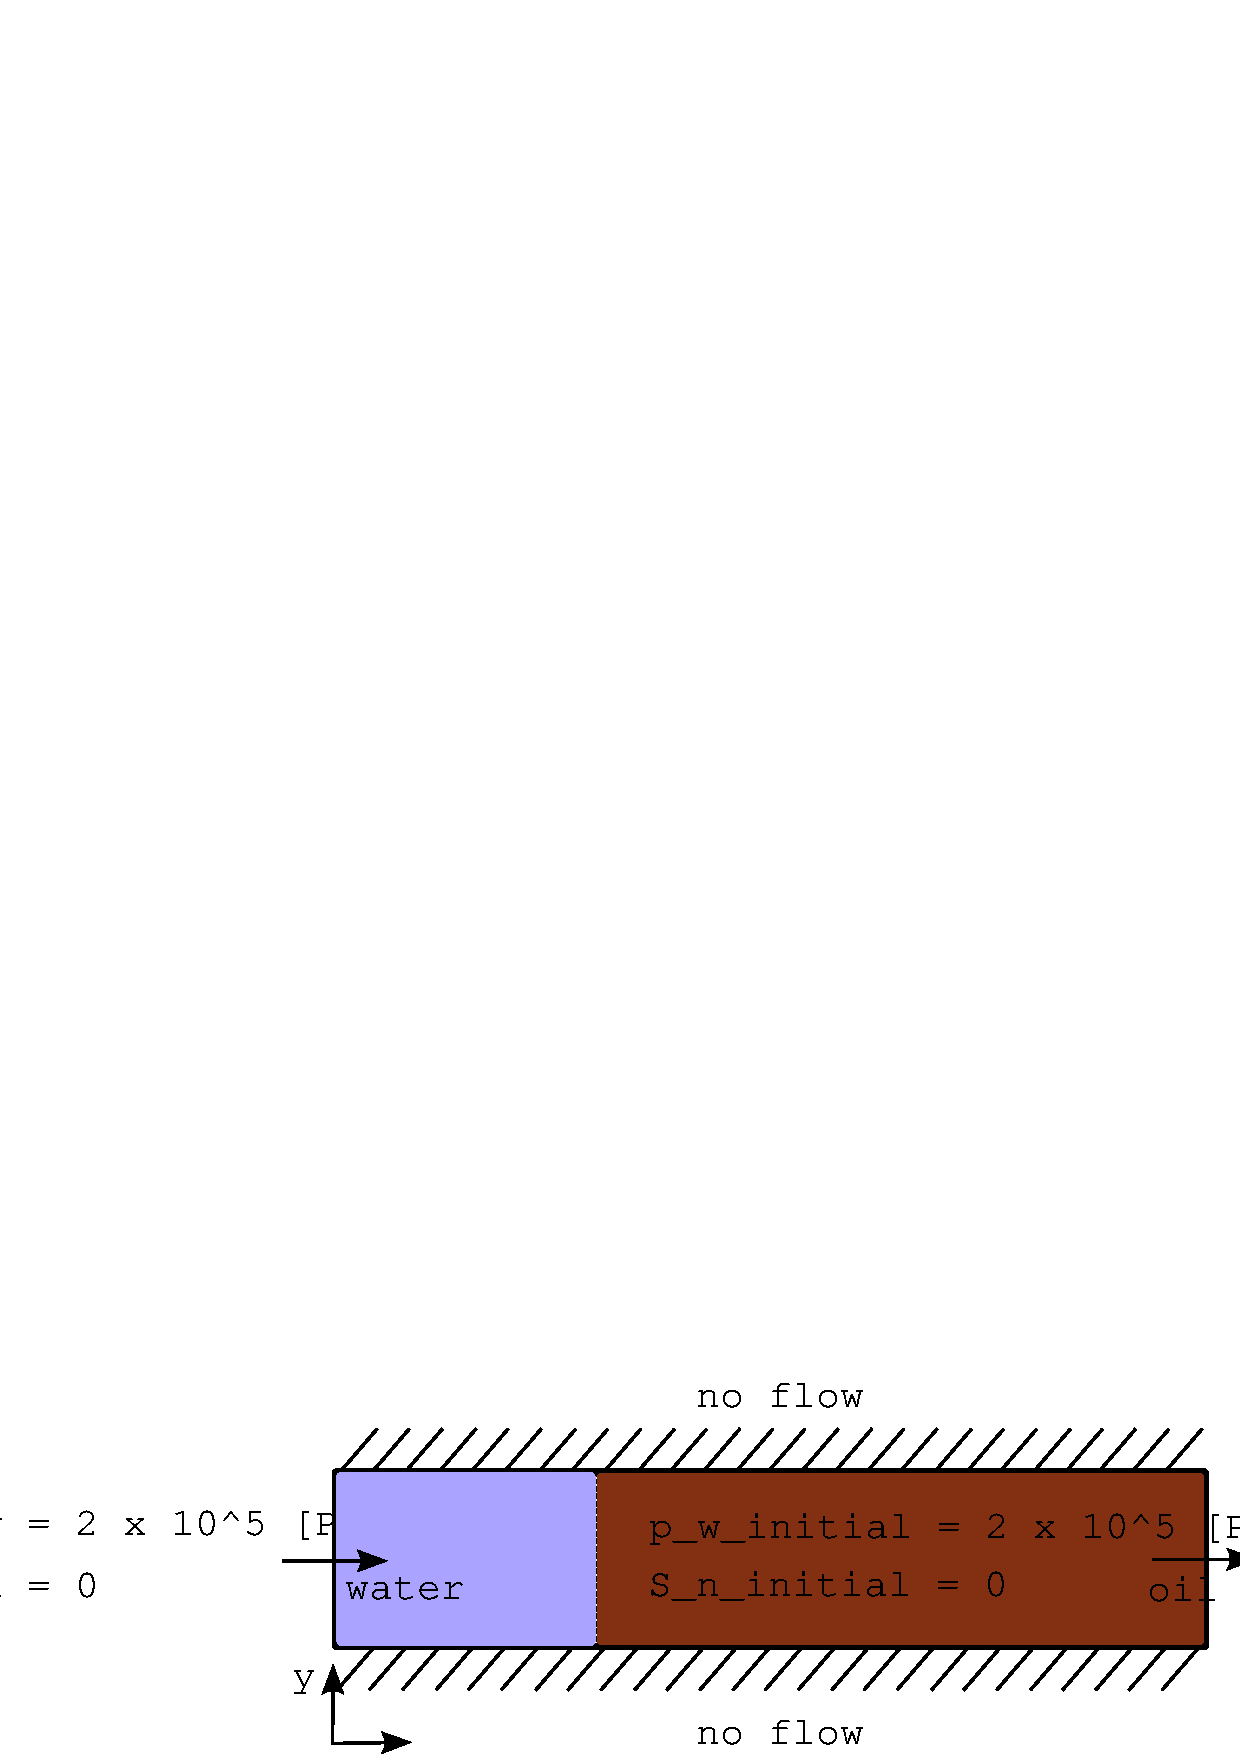
\includegraphics[width=0.9\linewidth,keepaspectratio]{EPS/tutorial-problemconfiguration}
\caption{Geometry of the tutorial problem with initial and boundary conditions.}\label{tutorial-decoupled:problemfigure}
\end{figure}

Listing \ref{tutorial-deoucpled:mainfile} shows how the main file, which has to be executed, has to be set up, if the problem described above is to be solved using a decoupled model. This main file can be found in the directory \texttt{/tutorial} of the stable part of \Dumux.

\begin{lst}[File tutorial/tutorial\_decoupled.cc]\label{tutorial-deoucpled:mainfile} \mbox{}
\lstinputlisting[basicstyle=\ttfamily\scriptsize,numbers=left, 
numberstyle=\tiny, numbersep=5pt]{../../tutorial/tutorial_decoupled.cc}
\end{lst}

First, from line \ref{tutorial-decoupled:include-begin} to line
\ref{tutorial-decoupled:include-end} the Dune and \Dumux files containing
essential functions and classes are included.

At line \ref{tutorial-decoupled:set-type-tag} the type tag of the
problem which is going to be simulated is set. All other data types
can be retrieved by the \Dumux property system and only depend on this
single type tag. Retrieving them is done between line
\ref{tutorial-decoupled:retrieve-types-begin} and
\ref{tutorial-decoupled:retrieve-types-end}. For an introduction to the
property system, see section \ref{sec:propertysystem}.

The first thing which should be done at run time is to initialize the
message passing interface using DUNE's \texttt{MPIHelper} class. Line
\ref{tutorial-decoupled:init-mpi} line is essential if the simulation is
intended to be run on more than one processor at the same time. Next,
the command line arguments are parsed starting at line
\ref{tutorial-decoupled:parse-args-begin} until line
\ref{tutorial-decoupled:parse-args-end}. In this case, we check if and
at which time a previous run of the simulation should be restarted, and we
parse the time when the simulation ends. As the maximum time-step in the 
sequential model is strictly bound by a CFL-criterion, the first time-step
size is initialized with the simulation time.

After this, a grid is created on line \ref{tutorial-decoupled:create-grid} 
and the problem is instantiated with information about the grid
(via its leaf grid view) on line \ref{tutorial-decoupled:instantiate-problem}.
If demanded, on line \ref{tutorial-decoupled:mainRestart} a state written to
disk by a previous simulation run is restored on request by the user.
Finally, the time manager controlling the simulation run is instantiated 
with the start parameters in line \ref{tutorial-decoupled:initTimeManager}
and the simulation proceedure is started by the time manager at line
\ref{tutorial-decoupled:execute}.



\subsection{The problem class} \label{decoupled_problem}

When solving a problem using \Dumux, the most important file is the
so-called \textit{problem file} as shown in listing
\ref{tutorial-decoupled:problemfile} of
\texttt{tutorialproblem\_decoupled.hh}.

\begin{lst}[File tutorial/tutorialproblem\_decoupled.hh]\label{tutorial-decoupled:problemfile} \mbox{}
\lstinputlisting[basicstyle=\ttfamily\scriptsize,numbers=left,
numberstyle=\tiny, numbersep=5pt, firstline=17]{../../tutorial/tutorialproblem_decoupled.hh}
\end{lst}

First, both \Dune  grid handlers and the decoupled model of \Dumux 
have to be included. Then, a new type tag is created for the problem 
on line \ref{tutorial-decoupled:create-type-tag}.  In this case, the 
new type tag inherits all properties defined for the \texttt{DecoupledTwoP} 
type tag, which means that for this problem the two-phase decoupled approach
is chosen as discretization scheme (defined via the include in line 
\ref{tutorial-decoupled:parent-problem}). On line \ref{tutorial-decoupled:set-problem}, 
a problem class is attached to the new type tag, while the grid which
is going to be used is defined on line \ref{tutorial-decoupled:set-grid-type} --
in this case an \texttt{SGrid} is created.  Since in Dune, there's no uniform
mechanism to allocate grids, the \texttt{Grid} property also contains
a static \texttt{create()} method which provides just that: From line 
\ref{tutorial-decoupled:grid-begin} to \ref{tutorial-decoupled:grid-end}, 
the geometry is defined and the grid is generated. The three variables of 
Type \texttt{Dune::FieldVector} define the lower left corner of the domain 
(\texttt{L}), the upper right corner of the domain (\texttt{H}) and the number 
of cells in $x$ and $y$ direction (\texttt{N}). The grid of type 
\texttt{Dune::SGrid} is then generated in line \ref{tutorial-decoupled:grid-end}. 
For more information about the dune grid interface, the different grid types 
that are supported and the generation of different grids it is referred to 
the \textit{Dune Grid Interface HOWTO} \cite{DUNE-HP}. 

Next, we select the material of the simulation: In case of a pure two-phase
model, each phase is a bulk fluid, and the complex (compositional) fluidsystems
do not need to be used. However, they can be used (see exercise 1 \ref{dec-ex1-fluidsystem}). 
Instead, we use a simplified fluidsystem container that provides classes 
for liquid and gas phases, line \ref{tutorial-decoupled:2p-system-start} to 
\ref{tutorial-decoupled:2p-system-end}. These are linked to the appropriate 
chemical species in line \ref{tutorial-decoupled:wettingPhase} and 
\ref{tutorial-decoupled:nonwettingPhase}. For all parameters that depend 
on space, such as the properties of the soil, the specific spatial parameters 
for the problem of interest are specified in line
\ref{tutorial-decoupled:set-spatialparameters}. 

Now we arrive at some model parameters of the applied two-phase decoupled 
model. Line \ref{tutorial-decoupled:velocityFormulation} defines that the 
wetting phase velocity rather than e.g. a total velocity is used for the 
transport system. As we regard capillary pressure, a capillary diffusive 
term is regarded, selected in line \ref{tutorial-decoupled:DiffusivePart}.
Line \ref{tutorial-decoupled:cfl} assigns the CFL-factor to be used in the
simulation run. The final property on line \ref{tutorial-decoupled:gravity} 
is optional and tells the model not to use gravity.

After all necessary information is written into the property system and 
its namespace is closed in line \ref{tutorial-decoupled:propertysystem-end},
the problem class is defined in line \ref{tutorial-decoupled:def-problem}. 
As its property, the problem class itsself is also derived from a parent, 
\texttt{IMPESProblem2P}. The class constructor (line 
\ref{tutorial-decoupled:constructor-problem}) is able to hold two vectors,
which is not needed in this tutorial.

Besides the definition of the boundary and initial conditions (discussed in 
subsection \label{decoupled-problem:boundary}), the problem class also contains
general information about the current simulation. First, the name used by
the \texttt{VTK-writer} to generate output is defined in the method of line
\ref{tutorial-decoupled:name}, and line \ref{tutorial-decoupled:restart} indicates
weather restart files are written. As decoupled schemes usually feature small 
timesteps, the method controlling the output in line \ref{tutorial-decoupled:output}
is very useful. The divisor of the modulo operation defines after how many timesteps
output should be written out -- the default ``1'' resembles output after each 
step.

The following methods all have in common that they may be dependent on space.
Hence, they all feature a common argument list:
\begin{itemize}
 \item \texttt{globalPos}: A vector holding the global Coordinates.
 \item \texttt{element} or \texttt{intersection}: Input for an iterator, that is 
    depending weather the parameter of the method is defined in an element, such as 
    initial values, or on an intersection, such as a boundary condition.
\end{itemize}
In the following, there are the methods for general parameters, source- or
sinkterms, boundary conditions (lines \ref{tutorial-decoupled:bctypePress} to
\ref{tutorial-decoupled:neumannSat}) and initial values for the transported
quantity in line \label{tutorial-decoupled:initSat}. For more information
on the functions, it is referred to the documentation in the code.

\subsection{The definition of the parameters that are dependent on space}\label{tutorial-decoupled:description-spatialParameters}

Listing \ref{tutorial-decoupled:spatialparametersfile} shows the file
\verb+tutorialspatialparameters_decoupled.hh+:

\begin{lst}[File tutorial/tutorialspatialparameters\_decoupled.hh]\label{tutorial-decoupled:spatialparametersfile} \mbox{}
\lstinputlisting[basicstyle=\ttfamily\scriptsize,numbers=left,
numberstyle=\tiny, numbersep=5pt, firstline=16]{../../tutorial/tutorialspatialparameters_decoupled.hh}
\end{lst}
As this file only slightly differs from the coupled version, it is referred to 
chapter \ref{tutorial-coupled:description-spatialParameters} for explanations.
However, as a standard Finite-Volume--scheme is used, in contrast to the box-method
in the coupled case, the argument list here is the same as for the problem 
functions:
\begin{itemize}
 \item \texttt{globalPos}: A vector holding the global Coordinates.
 \item \texttt{element}: Input for an element iterator, providing access
	to the current element of interest.
\end{itemize}

\subsection{Exercise}
\label{tutorial-deoucpled:exercises}
The following exercises will give you the opportunity to learn how you can change 
soil parameters, boundary conditions and fluid properties in \Dumux and to play along 
with the decoupled modelling framework.

\subsubsection{Exercise 1}
\renewcommand{\labelenumi}{\alph{enumi})}
For Exercise 1 you only have to make some small changes in the tutorial files.
\begin{enumerate}
\item \textbf{Altering output}
To get an impression what the results should look like you can first run the original version of the decoupled tutorial model by typing  \texttt{./tutorial\_decoupled 1e4}. The number behind the simulation name defines the timespan of the simulation run in seconds. For the visualisation with paraview please refer to \ref{quick-start-guide}.\\
As you can see, the simulation creates roughly 50 output files. To reduce these to perform longer simulations, change the method responsible for output in the file \texttt{tutorialproblem\_decoupled} to write an output only every 20 timesteps. Compile the main file by typing \texttt{make tutorial\_decoupled} and run the model. Now, run the simulation for 1e5 seconds.

\item \textbf{Changing the Model Domain and the Boundary Conditions} \\
Change the size of the model domain so that you get a rectangle
with edge lengths of x = 400 m \\  and y = 500 m and with discretisation lengths of  $\Delta \text{x} = 20$ m and $\Delta \text{y} = 20$ m. \\
Change the boundary conditions in the file \texttt{tutorialproblem\_decoupled.hh} so that water enters from the bottom and oil flows out at the top boundary. The right and the left boundary should be closed for water and oil fluxes.  \\

\item \textbf{Changing Fluids} \\
Now you can change the fluids. Use DNAPL instead of Oil and Brine instead of Water. To do that you have to select different components via the property system in the problem file:
\begin{enumerate}
 \item Brine: The class \texttt{Dumux::Brine} acts as a adapter to the fluid system that alters a pure water class by adding some salt. Hence, the class \texttt{Dumux::Brine} uses a pure water class, such as \texttt{Dumux::H2O}, as a second template argument after the data type \texttt{<Scalar>} as a template argument (be aware to use the complete water class with its own template parameter).
 \item DNAPL: A standard set of chemical substances is already included (via a list of \texttt{\#include ..} commandos) and hence easy accessible. This is not the case for the class \texttt{Dumux::SimpleDNAPL}, however, which is located in the folder \texttt{dumux/material/components/}. Try to include the file as well as select the component via the property system.
\end{enumerate}
If you want to take a closer look how the fluid classes are defined and which substances are already available please browse through the files in the directory
\texttt{/dumux/material/components}.

\item \textbf{Use the \Dumux fluid system}\label{dec-ex1-fluidsystem} \\
As you have experienced in the coupled tutorial (chapter \ref{tutorial-decoupled}), \Dumux usually organises fluid mixtures via a \texttt{fluidsystem}. This is also possible for the decoupled models: Uncomment, as we want to reuse it later on, the lines \ref{tutorial-decoupled:2p-system-start} to \ref{tutorial-decoupled:2p-system-end} in the problem file. If you use eclipse, this can easily be done by pressing \textit{str + shift + 7}, the same shortcut works to cancel the comment later on.\\
Now include the file \texttt{fluidsystems/h2o\_n2\_system.hh} in the material folder, and set a property \texttt{FluidSystem} with the appropriate type, \texttt{Dumux::H2O\_N2\_System<TypeTag>}. However, the complicated fluidsystem uses tabularized fluid data, which need to be initilized in the constructor body of the current problem by adding \texttt{GET\_PROP\_TYPE(TypeTag, PTAG(FluidSystem))::init();}, hence using the initialization function of the applied fluidsystem. As an alternative, use a simpler version of water, e.g. \texttt{Dumux::SimpleH2O}, and apply it for the property \texttt{Components} with type \texttt{H2O}. As water flow replacing a gas is much faster, test your simulation only until 1e4 seconds.\\
Please reverse the changes of this example, as we still use bulk phases and hence do not need such an extensive fluid system.
 
\item \textbf{Heterogeneities}  \\
Set up a model domain with the soil properties given in Figure \ref{tutorial-deoucpled:exercise1_d}. Adjust the boundary conditions so that water is again flowing from left to right.
\begin{figure}[h]
\psfrag{K1 =}{K $= 10^{-8}\text{ m}^2$}
\psfrag{phi1 =}{$\phi = 0.15$}
\psfrag{K2 =}{\textcolor{white}{K $= 10^{-9}\text{ m}^2$}}
\psfrag{phi2 =}{\textcolor{white}{$\phi = 0.3$}}
\psfrag{600 m}{600 m}
\psfrag{300 m}{300 m}
\centering
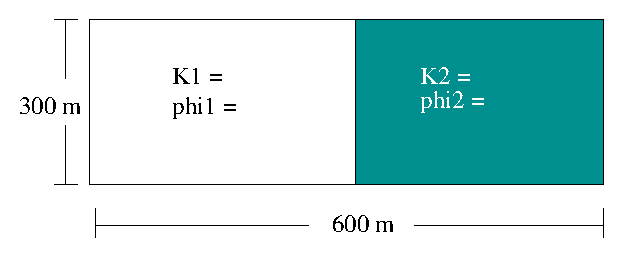
\includegraphics[width=0.5\linewidth,keepaspectratio]{EPS/exercise1_c.eps}
\caption{Exercise 1d: Set-up of a model domain a heterogeneity. $\Delta \text{x} = 20$ m $\Delta \text{y} = 20$ m.}\label{tutorial-deoucpled:exercise1_d}
\end{figure}
When does the front cross the material border? In paraview, the option \textit{View} $\rightarrow$ \textit{Animation View} is nice to get a rough feeling of the timestep sizes.
\end{enumerate}

\subsubsection{Exercise 2}
For this exercise you should create a new proplem file analogous to
the file \texttt{tutorialproblem\_decoupled.hh} and new spatial parameters 
just like \texttt{tutorialspatialparameters\_decoupled.hh}. These files need to
be included in the file \texttt{tutorial\_decoupled.cc}. 

The new file defining spatial parameters should contain the definition 
of a new class, such as \texttt{SpatialParametersEx2}. Make sure that you also adjust the guardian
macros in the header files (e.g. change \texttt{TUTORIALSPATIALPARAMETERS\_COUPLED} to
\texttt{SPATIALPARAMETERSEX2}). Besides also adjusting the guardian macros, 
the new problem file should define and use a new type tag for the problem as well as a new problem class
e.g. \texttt{ProblemEx2}. Make sure you assign your newly defined spatial 
parameter class to the \texttt{SpatialParameters} property for the new 
type tag. 

After this, change the \texttt{create()} method of the \texttt{Grid}
property so that it matches the domain described
by figure \ref{tutorial-decoupled:ex2_Domain}. Adapt the problem class
so that the boundary conditions are consistent with figure
\ref{tutorial-decoupled:ex2_BC}. Initially the domain is fully saturated
with water and the pressure is $p_w = 5 \times 10^5 \text{Pa}$ . Oil
infiltrates from the left side. Create a grid with $20$ cells in
$x$-direction and $10$ cells in $y$-direction. The simulation time
should be set to $6000 \text{s}$.

Now include your new problem file in the main file and replace the
\texttt{TutorialProblemCoupled} type tag by the one you've created and
compile the program.


\begin{figure}[h]
\psfrag{K1}{K $= 10^{-7}\text{ m}^2$}
\psfrag{phi1}{$\phi = 0.2$}
\psfrag{Lin}{Brooks Corey Law} 
\psfrag{Lin2}{$\lambda = 1.8$, $p_b = 1000$}
\psfrag{K2}{K $= 10^{-9}\text{ m}^2$}
\psfrag{phi2}{$\phi = 0.15$}
\psfrag{BC1}{Brooks Corey Law} 
\psfrag{BC2}{$\lambda = 2$, $p_b = 1500$}
\psfrag{H1y}{50 m}
\psfrag{H2y}{15 m}
\psfrag{H3y}{20 m}
\psfrag{L1x}{100 m}
\psfrag{L2x}{50 m}
\psfrag{L3x}{25 m}
\centering
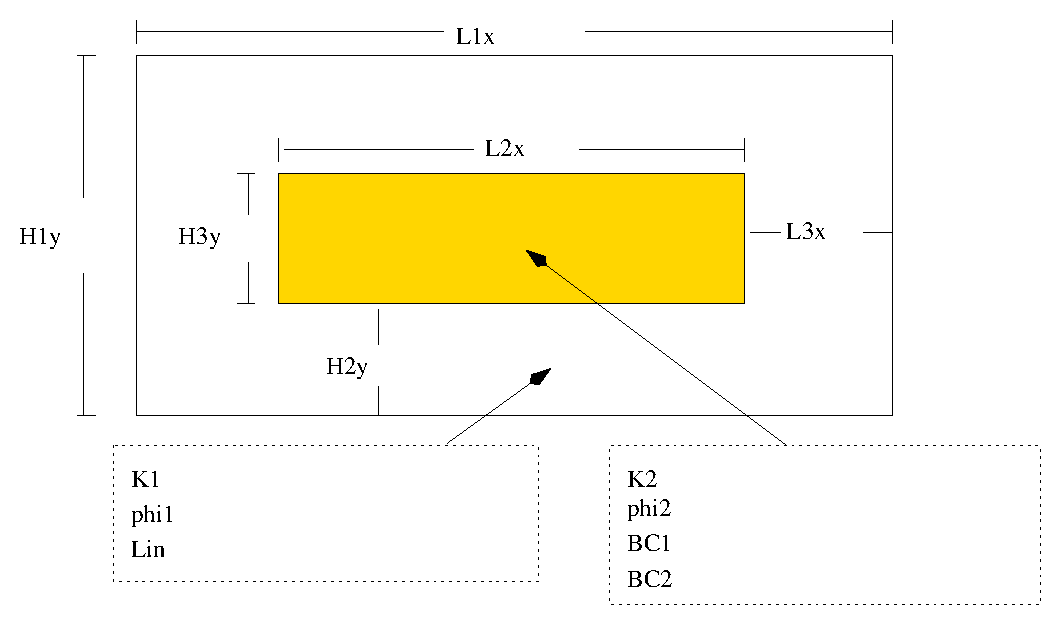
\includegraphics[width=0.8\linewidth,keepaspectratio]{EPS/Ex2_Domain.eps}
\caption{Set-up of the model domain and the soil parameters}\label{tutorial-decoupled:ex2_Domain}
\end{figure}

\begin{figure}[h]
\psfrag{pw}{$p_w = 5 \times 10^5$ \text{Pa}}
\psfrag{S}{$S_n = 1.0$}
\psfrag{qw}{$q_w = 2 \times 10^{-4}$ [kg/$\text{m}^2$s]}
\psfrag{qo}{$q_n = 0.0$ [kg/$\text{m}^2$s]}
\psfrag{no flow}{no flow}
\centering
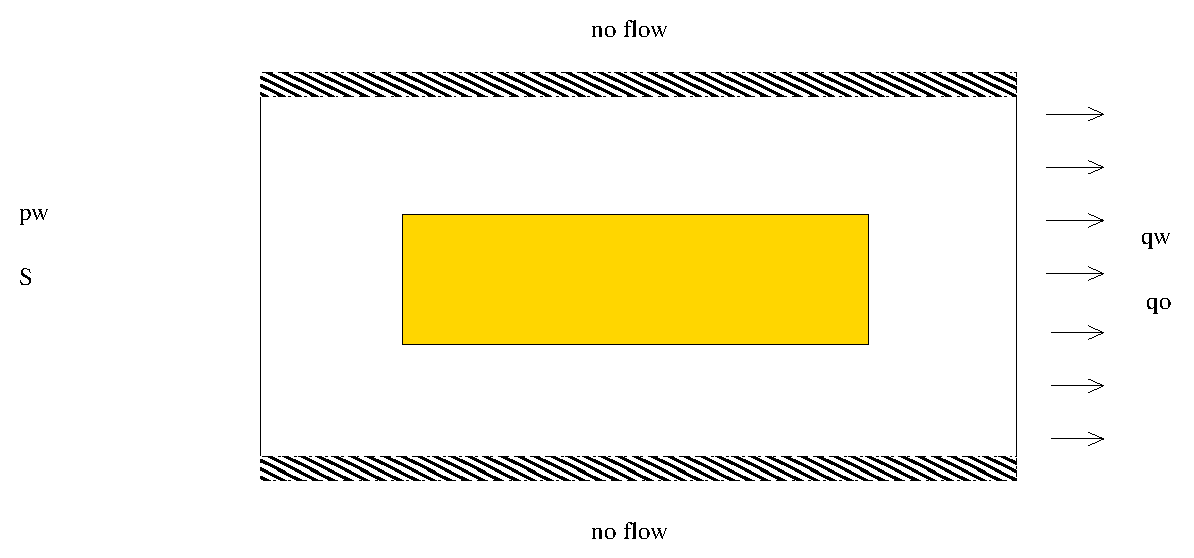
\includegraphics[width=0.8\linewidth,keepaspectratio]{EPS/Ex2_Boundary.eps}
\caption{Boundary Conditions}\label{tutorial-decoupled:ex2_BC}
\end{figure}

\begin{itemize}
 \item Investigate the saturation: Is the value range reasonable?
 \item What happens if you increase the resolution of the grid?
 \item Try out a CFL-factor of 1 and investigate the whole simulation run.
\end{itemize}


\subsubsection{Exercise 3}
Create a new file for benzene called \texttt{benzene.hh} and implement
a new fluid system. (You may get a hint by looking at existing fluid 
systems in the directory \verb+/dumux/new_material/fluidsystems+.)

Use benzene as a new fluid and run the model of Exercise 2 with water
and benzene. Benzene has a density of $889.51 \, \text{kg} / \text{m}^3$
and a viscosity of $0.00112 \, \text{Pa} \; \text{s}$. 

%%% Local Variables: 
%%% mode: latex
%%% TeX-master: "dumux-handbook"
%%% End: 

%\section[New model]{How to implement a new model}

TODO: describe how to impelment a new model
